\section{Low Rank}
\label{sec:LowRank}


\subsection{Upright orientation}
\label{subsec:upright orientation}

Most man-made models can be posed at a unique upright orientation which is consistent to human sense. Given a 3D digital model, finding its upright orientation and posing it at the right orientation is vital for users to recognize it. However, since produced by various techniques, digital man-made models, such as polygon meshes, might be sloped far from the upright orientation. So how to find the upright orientation would be an useful work.

\begin{figure*}[ht]
  \centering
  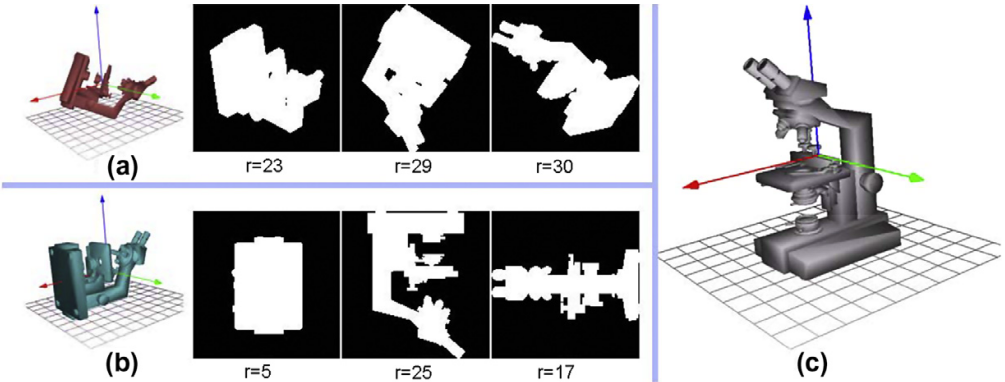
\includegraphics[width=6in]{images/lowrank}
  \caption{Low rank: observation. (a): local method\cite{jin2012unsupervised}. (b): global method\cite{wang2014upright}.}
\end{figure*}

Figure..shows the axis-aligned projections of an input man-made model with arbitrary(a) and axis-aligned orientation(b) onto the $y$-$z$, $y$-$z$ and $y$-$z$ plane(left to right) in the $x$-$y$-$z$(red-green-blue) coordinate system. Regarding these projections as two-domensional matrices, it is clear that the ranks of projection matrices in (b) are significantly $lower$ than those in (a). And, the upright orientation(c) should be one of the six orientations determined by the six axis-aligned candidate bases, i.e., top, bottom, left, right, front and back surface of the bounding box of the model. Briefly, ranks of projection matrices at axis-aligned orientations are lower than their counterparts at other orientations, since man-made models are mainly composed by horizonal and vertical edges and shapes.

\paragraph{(1)}Based on this observation, \cite{jin2012unsupervised} presents an unsupervised approach for finding the upright orientation of man-made models. Taking the $x$-$y$ plane projection as an example, they binarize the projection as black and white to generate the projection image $I$ with fixed resolution which can also be referred as a two-dimensional matrix. And to avoid affect of noise, $I$ can be modeled as a low-rank version $L$ with sparse-error matrix $E$: $I=L+E$. Then the problem is formulated as

\small{
\begin{equation}
 \label{eq:UprightJin}
 \min_{L,E,R}\|L\|_{*}+\lambda\|E\|_{1},~s.t.~I\circ R=L+E
\end{equation}
}
\\
where $\|\cdot\|_{*}$ and $\|\cdot\|_1$ are the nuclear norm(sum of all singular values) and the $L_1$ norm, which are closely related to rank of matrix and sparsity of matrix respectively. $R$ is a rigid rotation transformation matrix which is used to rectify $I$ to recover the optimal low-rank representation of $x$-$y$ plane projection from an arbitrary orientation. After selecting which projection should be rectified from $y$-$z$, $y$-$z$ and $y$-$z$, using () the man-made model will be aligned with some axes followed by final upright orientation selection from six orientations as mentioned above. However, whether a model fits for this algorithm depends on if the model contains dominant parts parallel to the supporting base, then it will fail if the model is composed by several equivalently main parts which have their own low-rank observation in different orientations.%This method can achieve great result when the model has perfect symmetries.

\paragraph{(2)}It is very natural to generalize this method in 3D space to construct three-order tensor(multidimensional array) with volume of the 3D model, i.e., the three-order tensor ought to have a $"$low rank$"$ behavior. \cite{wang2014upright} constructs this three-order tensor using the bounding box of the 3D model since the bounding box parallels the coordinate planes and contains the whole model. By translating the barycenter of the input model to the origin of the coordinate system, they just need to find and optimal rotation matrix $R$ to align the model with three axes by following optimization model

\small{
\begin{equation}
 \label{eq:UprightJin}
 R_{*}=\mathop{\argmin}_{R}(\|\chi(V\circ R)\|_{*})
\end{equation}
}
\\
where $V$ and $V\circ R$ respectively indicate the point coordinates of input model and the rotated model, $\chi(\cdot)$ is the three-order tensor. Similar to \cite{jin2012unsupervised}, after aligning the model with three axes, they select the upright orientation from six orientations by analyzing the geometric properties.
%
%But when a model has not any external symmetry or the symmetry in a big part whose rank plays the leading role in the low-rank optimization is in consistent with the model, the method may fail as well as \cite{jin2012unsupervised}.

\begin{figure}[ht]
  \centering
  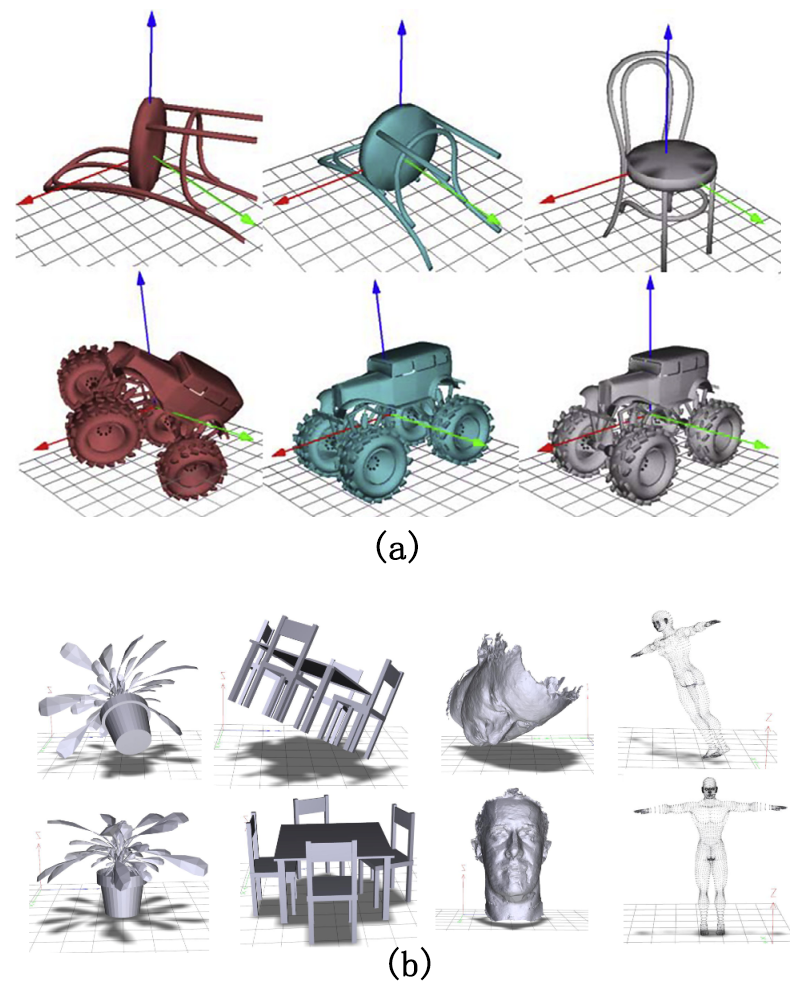
\includegraphics[width=3in]{images/upright_lowrank}
  \caption{Low rank: unsupervised upright orientation. (a): local method\cite{jin2012unsupervised}. (b): global method\cite{wang2014upright}.}
\end{figure} 